\begin{pastexam}[label={px:ccu-114-csb-07}]{中正資工所乙組 114 學年度 第 7 題}
（單選）

(5\%) What are the output value of the $\mathit{low}(v)$ for each vertex $v$ (in the order of $A, B, C, D, E, F, G, H, I$) in the given graph, when determining articulation points? As part of the process of computing depth-first numbers, you must start with vertex $A$ and select the one with the smaller alphabetical order first when performing the depth-first search.

\begin{center}
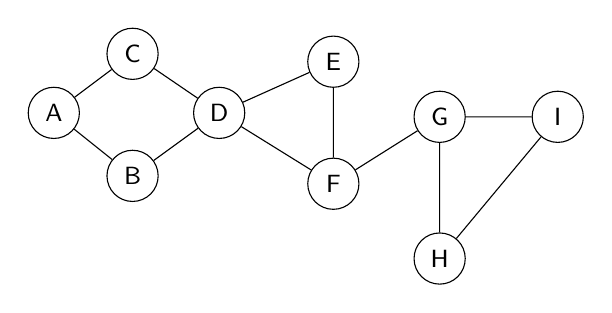
\begin{tikzpicture}[v/.style={circle,draw,minimum size=6.5mm,inner sep=0pt,font=\sffamily\small},x=1cm,y=1cm]
\node[v] (A) at (0,0) {A};
\node[v] (C) at (1.0,0.75) {C};
\node[v] (B) at (1.0,-0.8) {B};
\node[v] (D) at (2.1,0) {D};
\node[v] (E) at (3.55,0.65) {E};
\node[v] (F) at (3.55,-0.9) {F};
\node[v] (G) at (4.9,-0.05) {G};
\node[v] (I) at (6.4,-0.05) {I};
\node[v] (H) at (4.9,-1.85) {H};
\draw (A)--(C) (A)--(B) (C)--(D) (B)--(D) (D)--(E) (D)--(F) (E)--(F) (F)--(G) (G)--(H) (G)--(I) (H)--(I);
\end{tikzpicture}
\end{center}

\begin{enumerate}[label=\Alph*.]
\item (1, 1, 1, 1, 3, 3, 6, 6, 6)
\item (1, 1, 1, 1, 1, 1, 1, 1, 1)
\item (1, 1, 1, 3, 3, 3, 6, 6, 6)
\item (1, 1, 1, 3, 3, 3, 1, 1, 1)
\item None of the above
\end{enumerate}
\end{pastexam}

\begin{pastsoln}
答案是 E（None of the above）。 照題目規定的走法，$\mathit{low}$ 是 $(1, 1, 1, 1, 3, 3, 7, 7, 7)$；選項 A 的 $(1, 1, 1, 1, 3, 3, 6, 6, 6)$
是 $C$ 最後才拜訪時的結果，見最後一段。

做法照資結書第~23.5~節。 圖的鄰接（依字母排）：A：B, C；\ B：A, D；\ C：A, D；\ D：B, C, E, F；\ E：D, F；\ F：D, E, G；
\ G：F, H, I；\ H：G, I；\ I：G, H。

\textbf{DFS。} 從 A 出發，每次走字母最小的未拜訪鄰點，括號裡是 DFS 編號 $d$：
\begin{enumerate}
\item A(1) $\to$ B(2) $\to$ D(3)。 D 的鄰點裡 B 已拜訪，最小的未拜訪鄰點是 C。
\item D $\to$ C(4)。 C 的鄰點 A 已拜訪、不是父節點，C--A 是後向邊；D 是父節點。 C 結束，回到 D。
\item D $\to$ E(5) $\to$ F(6)。 F 的鄰點 D 已拜訪（F--D 是後向邊），E 是父節點，走 G。
\item F $\to$ G(7) $\to$ H(8) $\to$ I(9)。 I 的鄰點 G 已拜訪（I--G 是後向邊），H 是父節點。 一路退回 A。
\end{enumerate}
樹邊：A--B、B--D、D--C、D--E、E--F、F--G、G--H、H--I；後向邊：C--A、F--D、I--G。

\textbf{low 值}，從葉子往上（$\mathit{low}[u]$ 取 $d[u]$、子節點的 $\mathit{low}$、後向邊另一端的 $d$ 的最小值）：
\begin{center}
\begin{tabular}{cccl}
\toprule
頂點 & $d$ & 後向邊到 & $\mathit{low}$ \\
\midrule
I & 9 & G（7） & $\min(9, 7) = 7$ \\
H & 8 & --- & $\min(8, \mathit{low}[I] = 7) = 7$ \\
G & 7 & --- & $\min(7, \mathit{low}[H] = 7) = 7$ \\
F & 6 & D（3） & $\min(6, 3, \mathit{low}[G] = 7) = 3$ \\
E & 5 & --- & $\min(5, \mathit{low}[F] = 3) = 3$ \\
C & 4 & A（1） & $\min(4, 1) = 1$ \\
D & 3 & --- & $\min(3, \mathit{low}[C] = 1, \mathit{low}[E] = 3) = 1$ \\
B & 2 & --- & $\min(2, \mathit{low}[D] = 1) = 1$ \\
A & 1 & --- & $1$ \\
\bottomrule
\end{tabular}
\end{center}
依 A, B, \ldots, I 的順序是 $(1, 1, 1, 1, 3, 3, 7, 7, 7)$，不在 A--D 裡，選 E。

逐項檢查：
\begin{itemize}
\item A：$(1, 1, 1, 1, 3, 3, 6, 6, 6)$。 G、H、I 的 $\mathit{low}$ 等於 G 的 DFS 編號，要 G 的 $d = 6$，也就是 G 之前只拜訪了五個頂點。
這是 D 先走 E、F、G、H、I，最後才回頭拜訪 C 的走法（A 1、B 2、D 3、E 4、F 5、G 6、H 7、I 8、C 9）。 但在 D 的時候 C 比 E 小，
照規定要先走 C。 錯（若命題時 C 排在最後，預期答案會是 A）。
\item B：全部是 $1$，表示每個頂點的子樹都有後向邊回到 A，但 G、H、I 跟 A 之間沒有 F 以外的路，不可能。 錯。
\item C：$\mathit{low}[D] = 3$ 漏了 C--A 這條後向邊（C 在 D 的子樹裡）；G、H、I 的值也和上面一樣是 $6$ 而不是 $7$。 錯。
\item D：$\mathit{low}[G] = 1$ 不可能，G 的子樹裡沒有邊連到 F 以上。 錯。
\item E：正確的值不在選項中。 對。
\end{itemize}
不論哪一種走法，$\mathit{low}$ 和 $d$ 的大小關係相同，下一題的割點不受影響。
\end{pastsoln}
